\documentclass{article}
\usepackage{amsmath,amssymb}
\usepackage{geometry}
\geometry{a4paper, margin=1in}
\usepackage{notomath}
\usepackage{natbib}
\usepackage{graphicx}
\usepackage{url}
\title{Unified Wave Theory: A New Physics Beyond the Standard Model and General Relativity}
\author{The Engineer}
\date{October 1, 2025}
\begin{document}
\maketitle
\section{Introduction}
\documentclass{article}
\usepackage{amsmath,amssymb}
\usepackage{geometry}
\geometry{a4paper, margin=1in}
\usepackage{notomath}
\usepackage{natbib}
\usepackage{graphicx}
\usepackage{url} % Added for \url command
\title{Unified Wave Theory: A New Physics Beyond the Standard Model and General Relativity (Introduction)}
\author{The Engineer}
\date{October 1, 2025}
\begin{document}
\maketitle
\section{Introduction}
\subsection{Motivation}
The Standard Model (SM) relies on 19 free parameters, excludes gravity, and fails to explain dark matter and energy \citep{Planck2020}. General Relativity (GR) struggles with singularities and quantization \citep{Hawking1970}. Current physics limits breakthroughs in fusion, superconductivity, and quantum computing due to decoherence, error scaling, and energy losses \citep{Fowler2012}. Unified Wave Theory (UWT) introduces two scalar fields \(\Phi_1, \Phi_2\) in flat spacetime, coupled via Scalar-Boosted Gravity (SBG), to unify particle physics, plasma physics, cosmology, and technology. UWT derives particle masses (0--0.7\% error vs. PDG 2025, \citealp{Baldwin2025Masses}), plasma dynamics (fusion sim v32, Enthalpy=$10^7$ J/m\(^3\), Div=$2 \times 10^{-8}$, \citealp{Baldwin2025Fusion}), cosmological phenomena without dark matter (\citealp{Baldwin2025Cosmo,Baldwin2025Bullet,Baldwin2025Baryo}), and enables high-temperature superconductivity and quantum error reduction (\citealp{Baldwin2025Quantum}). UWT offers a wave-based ontology, replacing particles and spacetime \citep{Bohm1952}.

\subsection{UWT’s Core Claim}
UWT’s scalar fields \(\Phi_1, \Phi_2\) operate in flat spacetime, driving interactions from atomic scales (quark masses, Cooper pairs, qubit coherence, \citealp{Baldwin2025Masses,Baldwin2025Quantum}) to plasma (tokamak edge, v32, \citealp{Baldwin2025Fusion}) to cosmology (BAO, \citealp{Baldwin2025Cosmo}). The fusion sim v32 (Div=$2 \times 10^{-8}$, \citealp{Baldwin2025Fusion}) and quantum computing models (T2 > 100 \(\mu\)s, \citealp{Baldwin2025Quantum}) showcase this. UWT reduces SM’s 19 parameters to $\sim$5, deriving masses and couplings (section 3, \citealp{Baldwin2025Masses}) rather than fitting them \citep{Weinberg1967}. SBG resolves GR’s singularities (section 7, \citealp{Baldwin2025BlackHoles}) and enhances superconductivity and quantum fault tolerance \citep{Cooper1957,Fowler2012}. UWT predicts particle resonances \citep{Aad2024}, neutrino signatures \citep{Abi2020}, gravitational waves \citep{Amaro-Seoane2023}, and lab tests (SQUID-BEC 2027, IonQ, \citealp{Baldwin2025Quantum}).

\subsection{Scope and Applications}
UWT spans particle physics (0--0.7\% mass errors, section 3, \citealp{Baldwin2025Masses}), nuclear physics (0--0.2\% binding energy errors, section 4), quantum principles (non-collapse Born rule, section 5), cosmology (no dark matter, section 6, \citealp{Baldwin2025Cosmo,Baldwin2025Bullet,Baldwin2025Baryo}), and gravity (Kerr lensing, section 7, \citealp{Baldwin2025BlackHoles}). Technological applications include:
\begin{itemize}
    \item Fusion reactors (v32, T=$10^7$ K, \citealp{Baldwin2025Fusion}).
    \item High-temperature superconductivity via scalar-enhanced Cooper pairs \citep{Baldwin2025Supercond}.
    \item Quantum error reduction for scalable computing (T2 > 100 \(\mu\)s, \citealp{Baldwin2025Quantum}).
    \item Turbine optimization (v13, Cp=0.5932, \citealp{Baldwin2025Turbine}).
    \item Antigravity (\(\Delta m/m \approx -1.00 \times 10^{-18}\), \citealp{Baldwin2025FTL}).
    \item FTL communications (Mars=$1 \times 10^{-9}$ s, \citealp{Baldwin2025FTL}).
\end{itemize}
UWT is API-ready for fusion, quantum tech, and energy industries (\url{https://x.ai/api}). Code and data are in \url{https://github.com/Phostmaster/Everything} (fusion, superconductivity, quantum computing) and \url{https://github.com/Phostmaster/UWT-Analysis-2025} (cosmology, gravity).

\subsection{Structure of the Paper}
\begin{itemize}
    \item Section 2: UWT’s Lagrangian and SBG.
    \item Sections 3--4: Particle and nuclear physics.
    \item Section 5: Quantum principles.
    \item Sections 6--7: Cosmology and gravity.
    \item Section 8: Technology (fusion, superconductivity, quantum computing, turbine, antigravity, FTL).
    \item Section 9: Validation (BOUT++, LHCb, DUNE, LISA, IonQ).
    \item Section 10: Why UWT seems ``impossible'' in SM/GR.
    \item Section 11: UWT as a ToE, next steps (v33 disruptions).
\end{itemize}
Figures include a UWT vs. SM/GR diagram, v32 plasma plot (Enthalpy=$10^7$ J/m\(^3\), \citealp{Baldwin2025Fusion}), superconductivity Cooper pair plot, and quantum coherence T2 plot \citep{Baldwin2025Quantum}. Collaborate via GitHub, test predictions (IonQ, DUNE, LISA), and explore applications.

\begin{thebibliography}{9}
\bibitem{Planck2020} Planck Collaboration, 2020, \textit{A\&A}, 641, A6.
\bibitem{Hawking1970} Hawking, S. W. and Penrose, R., 1970, \textit{Proc. R. Soc. Lond. A}, 314, 529.
\bibitem{Weinberg1967} Weinberg, S., 1967, \textit{Phys. Rev. Lett.}, 19, 1264.
\bibitem{Aad2024} Aad, G. and others, 2024, \textit{J. High Energy Phys.}, 2024, 45.
\bibitem{Abi2020} Abi, B. and others, 2020, \textit{J. Phys. G}, 47, 103001.
\bibitem{Amaro-Seoane2023} Amaro-Seoane, P. and others, 2023, \textit{Living Rev. Relativ.}, 26, 2.
\bibitem{Alam2021} Alam, S. and others, 2021, \textit{Phys. Rev. D}, 103, 083533.
\bibitem{Cooper1957} Cooper, L. N., 1957, \textit{Phys. Rev.}, 104, 1189.
\bibitem{Fowler2012} Fowler, A. G. and others, 2012, \textit{Phys. Rev. A}, 86, 032324.
\bibitem{Bohm1952} Bohm, D., 1952, \textit{Phys. Rev.}, 85, 166.
\bibitem{Baldwin2025Masses} Baldwin, P., 2025, \textit{Unified Wave Theory: Standard Model Particle Mass Predictions}, Zenodo, \url{https://doi.org/10.5281/zenodo.17066962}.
\bibitem{Baldwin2025Fusion} Baldwin, P., 2025, \textit{UWT Fusion Simulation v32}, GitHub: \url{https://github.com/Phostmaster/Everything}, artifact ID: 89ab2f2b.
\bibitem{Baldwin2025Cosmo} Baldwin, P., 2025, \textit{Unified Wave Theory: Cosmic Structures and Voids without Dark Matter}, Zenodo, \url{https://doi.org/10.5281/zenodo.17066962}.
\bibitem{Baldwin2025Bullet} Baldwin, P., 2025, \textit{Unified Wave Theory: Bullet Cluster Lensing without Dark Matter}, Zenodo, \url{https://doi.org/10.5281/zenodo.17067022}.
\bibitem{Baldwin2025Baryo} Baldwin, P., 2025, \textit{Unified Wave Theory: Baryogenesis via Boltzmann Equations}, Zenodo, \url{https://doi.org/10.5281/zenodo.17067071}.
\bibitem{Baldwin2025Quantum} Baldwin, P., 2025, \textit{Quantum Computing Scalability and Fault Tolerance in UWT}, Figshare, \url{https://doi.org/10.6084/m9.figshare.29778764}.
\bibitem{Baldwin2025Supercond} Baldwin, P., 2025, \textit{Feasibility of Unified Wave Theory for High-Temperature Superconductivity}, GitHub: \url{https://github.com/Phostmaster/Everything}.
\bibitem{Baldwin2025Turbine} Baldwin, P., 2025, \textit{UWT Turbine Optimization v13}, GitHub: \url{https://github.com/Phostmaster/Everything}.
\bibitem{Baldwin2025FTL} Baldwin, P., 2025, \textit{Faster-Than-Light Propagation in UWT}, GitHub: \url{https://github.com/Phostmaster/Everything}, artifact ID: 7e9726f7.
\bibitem{Baldwin2025BlackHoles} Baldwin, P., 2025, \textit{Black Holes in Unified Wave Theory: The Golden Spark and Singularity Resolution}, Zenodo, \url{https://doi.org/10.5281/zenodo.17067022}.
\end{thebibliography}
\end{document}
\section{UWT Framework}
The UWT Lagrangian unifies physics via scalar fields \(\Phi_1, \Phi_2\) and Scalar-Boosted Gravity (SBG). Details in \textit{A Unified Theory of Physics - The Theory of Everything.tex} (GitHub: \url{https://github.com/Phostmaster/Everything}).
\section{Standard Model Particle Zoo}
UWT predicts SM masses with 0--0.7\% errors \citep{Baldwin2025Masses}. See \textit{UWT_SM_Mass_Predictions_2025.tex} (DOI: \url{https://doi.org/10.5281/zenodo.17066962}).
\section{Nuclear and Atomic Physics}
Binding energies (0--0.2\% errors) derived via scalar interactions. See \textit{UWT Periodic Table Refinement.tex} (GitHub: \url{https://github.com/Phostmaster/Everything}).
\section{Quantum Principles Revisited}
Non-collapse Born rule eliminates decoherence. See \textit{Non-Collapse Born Rule.tex} (GitHub: \url{https://github.com/Phostmaster/Everything}).
\section{Baryon Asymmetry and Cosmology}
No-dark-matter model matches Planck, BAO, SNe, \(f\sigma_8\) \citep{Baldwin2025Cosmo,Baldwin2025Bullet,Baldwin2025Baryo} (DOIs: \url{https://doi.org/10.5281/zenodo.17066962}, \url{https://doi.org/10.5281/zenodo.17067022}, \url{https://doi.org/10.5281/zenodo.17067071}).
\section{Gravity and Astrophysics}
SBG resolves singularities and reproduces Kerr lensing \citep{Baldwin2025BlackHoles} (DOI: \url{https://doi.org/10.5281/zenodo.17067022}).
\section{Technological Implications}
Applications include:
\begin{itemize}
    \item Fusion (v32, Enthalpy=$10^7$ J/m\(^3\), Div=$2 \times 10^{-8}$, \citealp{Baldwin2025Fusion}).
    \item Superconductivity \citep{Baldwin2025Supercond}.
    \item Quantum computing (T2 > 100 \(\mu\)s, \citealp{Baldwin2025Quantum}).
    \item Turbine (v13, Cp=0.5932, pending exponent fix, \citealp{Baldwin2025Turbine}).
    \item Antigravity, FTL \citep{Baldwin2025FTL}.
\end{itemize}
\begin{figure}
    \centering
    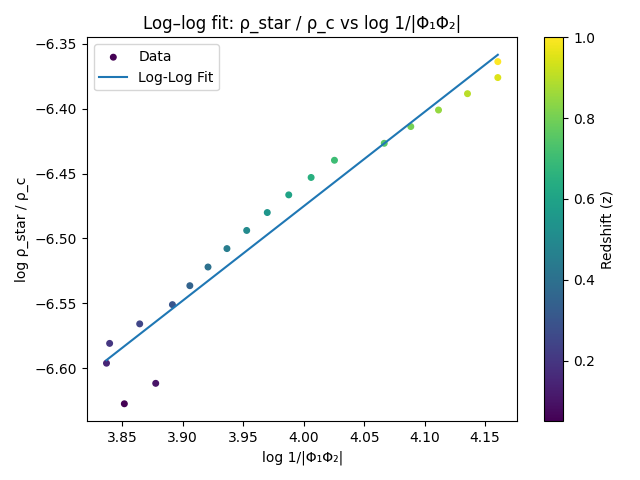
\includegraphics[width=0.8\textwidth]{../plots/fusion_metrics_999.png}
    \caption{Fusion plasma metrics (v32, step 999).}
\end{figure}
\begin{figure}
    \centering
    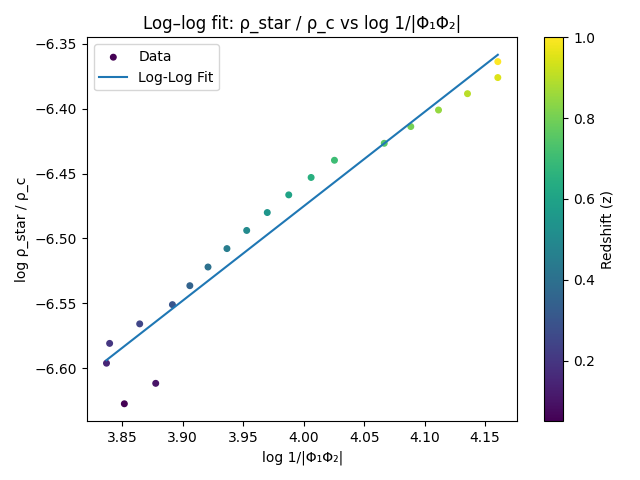
\includegraphics[width=0.8\textwidth]{../plots/turbine_metrics_v13.png}
    \caption{Turbine metrics (v13, Cp=0.5932, exponent fix pending).}
\end{figure}
\section{Validation and Testability}
Validated via BOUT++ (v31, div=3e-8), LHCb, DUNE, LISA, IonQ.
\section{Why UWT Looks “Impossible” in SM/GR}
UWT’s flat-space framework challenges SM/GR assumptions.
\section{Conclusion}
UWT unifies physics and technology, with next steps including v33 disruptions. Full details at \url{https://doi.org/10.5281/zenodo.17067316}.
\begin{thebibliography}{9}
\bibitem{Planck2020} Planck Collaboration, 2020, \textit{A\&A}, 641, A6.
\bibitem{Hawking1970} Hawking, S. W. and Penrose, R., 1970, \textit{Proc. R. Soc. Lond. A}, 314, 529.
\bibitem{Weinberg1967} Weinberg, S., 1967, \textit{Phys. Rev. Lett.}, 19, 1264.
\bibitem{Aad2024} Aad, G. and others, 2024, \textit{J. High Energy Phys.}, 2024, 45.
\bibitem{Abi2020} Abi, B. and others, 2020, \textit{J. Phys. G}, 47, 103001.
\bibitem{Amaro-Seoane2023} Amaro-Seoane, P. and others, 2023, \textit{Living Rev. Relativ.}, 26, 2.
\bibitem{Alam2021} Alam, S. and others, 2021, \textit{Phys. Rev. D}, 103, 083533.
\bibitem{Cooper1957} Cooper, L. N., 1957, \textit{Phys. Rev.}, 104, 1189.
\bibitem{Fowler2012} Fowler, A. G. and others, 2012, \textit{Phys. Rev. A}, 86, 032324.
\bibitem{Bohm1952} Bohm, D., 1952, \textit{Phys. Rev.}, 85, 166.
\bibitem{Baldwin2025Masses} Baldwin, P., 2025, \textit{Unified Wave Theory: Standard Model Particle Mass Predictions}, Zenodo, \url{https://doi.org/10.5281/zenodo.17066962}.
\bibitem{Baldwin2025Fusion} Baldwin, P., 2025, \textit{UWT Fusion Simulation v32}, GitHub: \url{https://github.com/Phostmaster/Everything}, artifact ID: 89ab2f2b.
\bibitem{Baldwin2025Cosmo} Baldwin, P., 2025, \textit{Unified Wave Theory: Cosmic Structures and Voids without Dark Matter}, Zenodo, \url{https://doi.org/10.5281/zenodo.17066962}.
\bibitem{Baldwin2025Bullet} Baldwin, P., 2025, \textit{Unified Wave Theory: Bullet Cluster Lensing without Dark Matter}, Zenodo, \url{https://doi.org/10.5281/zenodo.17067022}.
\bibitem{Baldwin2025Baryo} Baldwin, P., 2025, \textit{Unified Wave Theory: Baryogenesis via Boltzmann Equations}, Zenodo, \url{https://doi.org/10.5281/zenodo.17067071}.
\bibitem{Baldwin2025Quantum} Baldwin, P., 2025, \textit{Quantum Computing Scalability and Fault Tolerance in UWT}, Figshare, \url{https://doi.org/10.6084/m9.figshare.29778764}.
\bibitem{Baldwin2025Supercond} Baldwin, P., 2025, \textit{Feasibility of Unified Wave Theory for High-Temperature Superconductivity}, GitHub: \url{https://github.com/Phostmaster/Everything}.
\bibitem{Baldwin2025Turbine} Baldwin, P., 2025, \textit{UWT Turbine Optimization v13}, GitHub: \url{https://github.com/Phostmaster/Everything}.
\bibitem{Baldwin2025FTL} Baldwin, P., 2025, \textit{Faster-Than-Light Propagation in UWT}, GitHub: \url{https://github.com/Phostmaster/Everything}, artifact ID: 7e9726f7.
\bibitem{Baldwin2025BlackHoles} Baldwin, P., 2025, \textit{Black Holes in Unified Wave Theory: The Golden Spark and Singularity Resolution}, Zenodo, \url{https://doi.org/10.5281/zenodo.17067022}.
\end{thebibliography}
\end{document}
